
The source can be found at \url{http://cs.au.dk/~ptx/SpinOff.tgz}

After starting the program, the simulation is paused. It can be
started by changing the setting ``running'' in the settings dialog.

Initially, the $M$ field is parallel to the $B_0$ field, so nothing
will happen when the simulator is running. The next setting ``Run FID
sequence'' will move the $M$ field to the $xy$-plane, and the spin
will start to decay into the direction of $B_0$.

As the simulator is running, a grid of images are showing the status
(fig. \ref{fig:spinoff}). At index (0,0) (the lower left corner) the
input image is shown.

% If the user press ``k'', the images at (1,0) and (2,0) will show the
% fourier transformation and the inverse.

The image at (0,1) represents the spin at each point. The red, green
and blue component of the image represents $M_x$,$M_y$ and $M_z$.

The recorded signal is shown in (2,1), and a plot of the last line is
shown in (2,2).

\begin{figure*}
  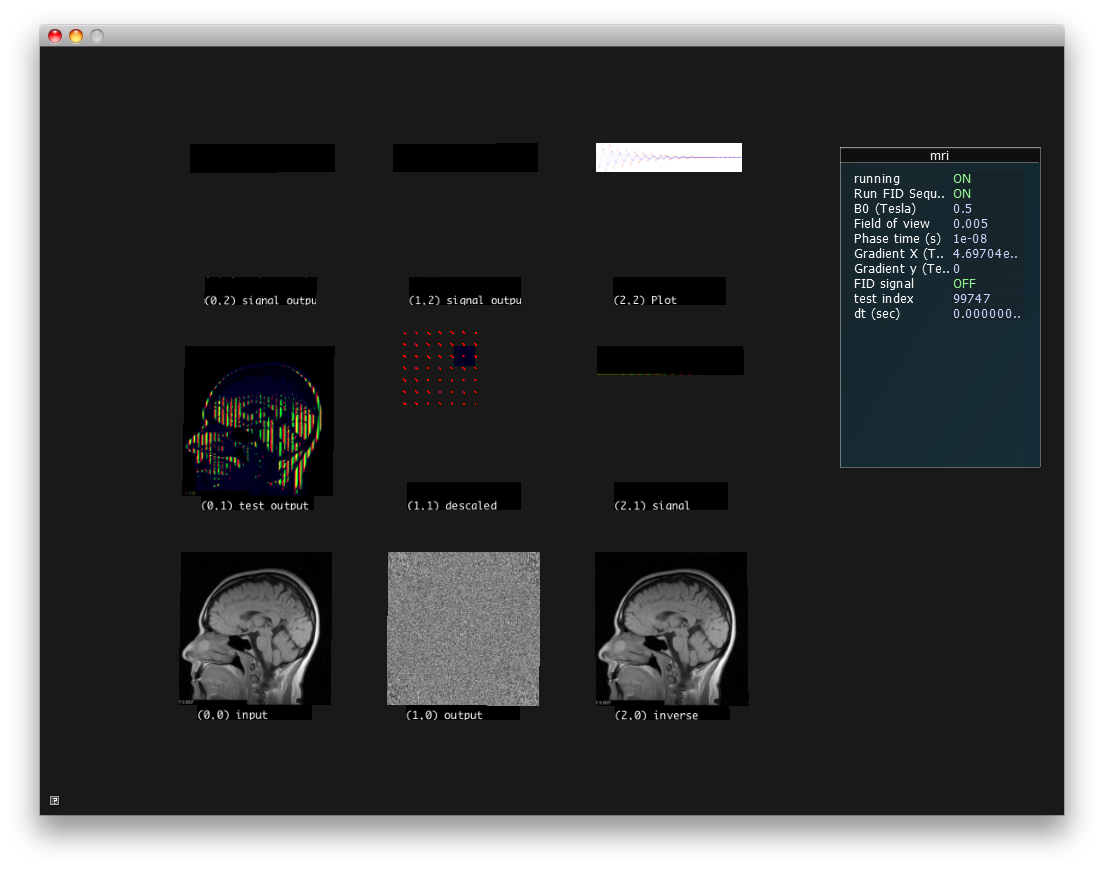
\includegraphics[width=\textwidth]{spinoff.png}
  \caption{Simulator}
  \label{fig:spinoff}
\end{figure*}

%%% Local Variables: 
%%% mode: latex
%%% TeX-master: "report"
%%% End: 
